\documentclass{article}

\usepackage[margin=0.5in]{geometry}
\usepackage[czech]{babel}
\usepackage{graphicx}
\usepackage{booktabs}
\usepackage[texMathDollars,pipeTables=true,tableCaptions,hybrid]{markdown}

\begin{document}

\begin{center}
  \Large \bfseries
Logistická rovnice
\end{center}
\pagestyle{empty}


\begin{markdown}

Modelem pro růst populací v prostředí s nosnou kapacitou prostředí, který je
všeobecně přijímán jako vhodný kompromis mezi přesností popisu a matematickou
jednoduchostí je Verhulst-Pearlův model růstu.

# Předpoklady

* Rychlost růstu populace vztažená na jedince (per-capita) klesá vlivem vnitrodruhové konkurence.
* Pro jednoduchost předpokládáme lineární pokles, který se zastaví při dosažení nosné kapacity.
* Jinými slovy toto znamená, že rychlost růstu populace v prostředí s omezenou nosnou kapacitou je úměrná současně 
velikosti této populace a volnému místu v životním prostředí vyjádřenému procentem z obsazené nosné kapacity.


# Model a výstup z modelu


\end{markdown}

\begin{minipage}[t]{0.5\linewidth}
V prostředí o nosné kapacita prostředí $K$ modeluje vývoj populace o
velikosti $x$ rovnice
$$\frac{\mathrm dx}{\mathrm dt}=rx\left(1-\frac xK\right),$$ kde $r$
je per-capita rychlostí růstu bez započtení konkurence.

Bez újmy na obecnosti (resp. po vhodné volbě jednotky času a jednotky
velikosti populace) je možno klást $r=K=1$.


\end{minipage}\begin{minipage}[t]{0.5\linewidth}
  \vspace*{-20pt}
  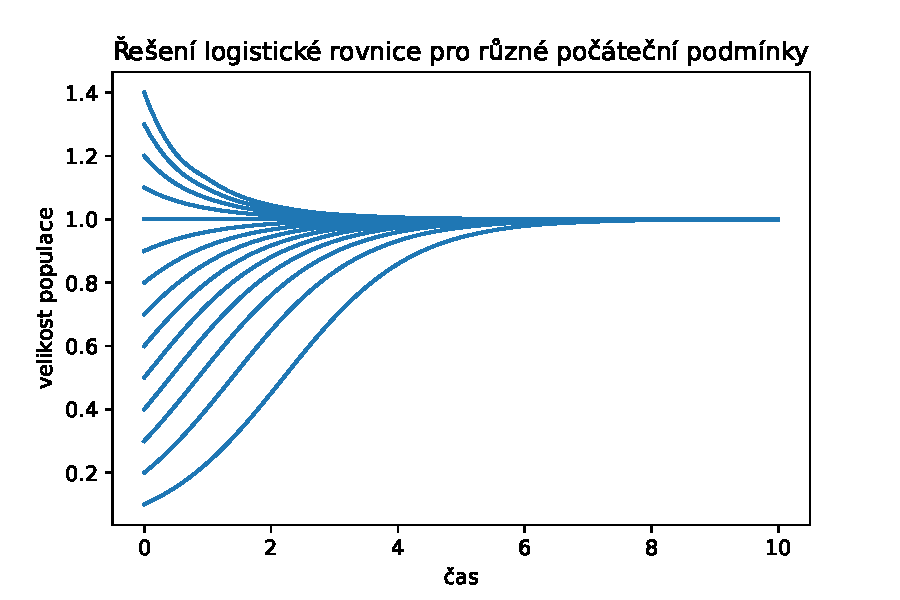
\includegraphics[width=\linewidth]{logisticka.pdf}
\end{minipage}

\begin{markdown}

# Možné modifikace

Logistická rovnice je základní rovnice pro modelování populací. Mnoho obecnějších modelů z této rovnice vychází.

\end{markdown}

\begin{minipage}[t]{0.45\linewidth}
  \vspace*{0pt}
\everymath{\displaystyle}
\begin{tabular}{ll}
  \toprule
  Modifikace&Tvar rovnice\\
  \midrule
Alleeho efekt & $\frac{\mathrm dx}{\mathrm dt}=rx\left(1-\frac xK\right)\left(\frac
xA-1\right)$\\[5mm]
Lov konstantní intenizity & $\frac{\mathrm dx}{\mathrm dt}=rx\left(1-\frac xK\right)-h$\\[5mm]
Lov s konstantním úsilím & $\frac{\mathrm dx}{\mathrm dt}=rx\left(1-\frac xK\right)-hx$\\[5mm]
Populace vystavená predaci & $\frac{\mathrm dx}{\mathrm dt}=rx\left(1-\frac xK\right)-f(x)y$\\[5mm]
  Konkurence populací & $\begin{cases}
                        \begin{aligned}
           \frac{\mathrm dx}{\mathrm dt}=rx\left(1-\frac {x-\alpha y}K\right)\\
           \frac{\mathrm dy}{\mathrm dt}=ry\left(1-\frac {y-\beta x}K\right)
                        \end{aligned}
\end{cases}
$\\
  \bottomrule
\end{tabular}

\end{minipage}\hfill
\begin{minipage}[t]{0.45\linewidth}
  \vspace*{0pt}

  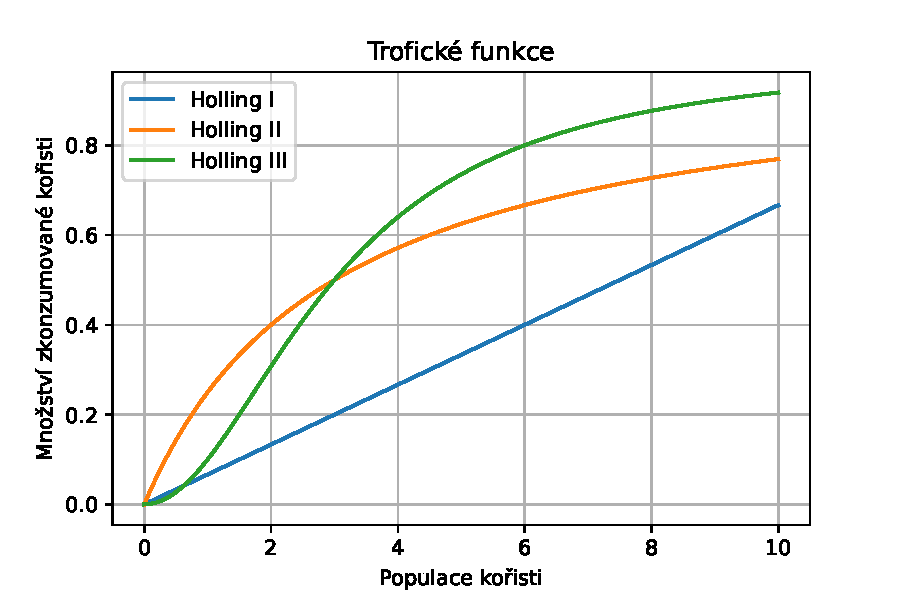
\includegraphics[width=\linewidth]{holling.pdf}

  \vspace*{0pt}
\end{minipage}


\bigskip
V tabulce jsou $x$ a $y$ velikosti populací a $f(x)$ je trofická funkce dravců. Ostatní parametry jsou zpravidla konstanty.
Trofické funkce rozlišujeme podle toho, jaké je chování kořisti, možnosti jejího úkrytu, jaká je strategie predátora a podobně (viz obrázek).
\end{document}


%%% Local Variables: 
%%% TeX-command-extra-options: "-shell-escape"
%%% End:
